\documentclass[11pt,a4paper]{article}
\usepackage[a4paper,top=14mm,bottom=14mm,left=15mm,right=15mm]{geometry}
\usepackage[T1]{fontenc}
\usepackage{amsmath}
\usepackage{amssymb}
\usepackage{array}
\usepackage{multicol}
\usepackage{tikz}
\usetikzlibrary{arrows.meta}

% ================================================================
% Inequalities: revision questions.
%
% Two pages of questions, in black and white, with a heading for each
% topic on the Maths Revision topic list in the same order. Each topic
% has a few short questions that start easy, with a diagram only where
% a question uses one, and the sheet ends with some problem solving.
% There are no key facts or worked examples on the sheet: the methods
% are in the worked solutions and the revision guide. Questions are
% numbered through the sheet so that the answer key and the worked
% solutions can refer to them.
% ================================================================

\pagestyle{empty}
\setlength{\parindent}{0pt}
\setlength{\parskip}{2pt}
\setlength{\columnsep}{9mm}

% A topic from the revision list.
\newcommand{\topic}[1]{\par\addvspace{14pt}{\bfseries #1}\par\nobreak\vspace{2pt}}

% Questions are numbered through the whole sheet.
\newcounter{qn}
\newcommand{\q}{\par\addvspace{9pt}\stepcounter{qn}\hangindent=1.6em\hangafter=1\noindent
  \makebox[1.6em][l]{\textbf{\theqn}}}

% \numline{<label>}{<drawing>}: a number line from -4 to 5, with the
% drawing placed at height 4, above the line.
\newcommand{\numline}[2]{%
  \begin{tikzpicture}[x=6.5mm,y=1mm]
    \node[anchor=east] at (-4.9,0) {#1};
    \draw[{Stealth[length=1.5mm]}-{Stealth[length=1.5mm]}] (-4.6,0) -- (5.6,0);
    \foreach \n in {-4,...,5}{\draw (\n,-1) -- (\n,1); \node[below,font=\small] at (\n,-1) {$\n$};}
    #2
  \end{tikzpicture}}
\newcommand{\opencircle}[1]{\draw[thick,fill=white] (#1,4) circle (1.2mm);}
\newcommand{\filledcircle}[1]{\fill (#1,4) circle (1.2mm);}

% \smallgraph{<shading>}{<boundary line>}: axes from -2 to 4. The grid is
% drawn over the shading, and the boundary line over the grid.
\newcommand{\smallgraph}[2]{%
  \begin{tikzpicture}[x=4.6mm,y=4.6mm,font=\scriptsize]
    #1
    \draw[black!25,step={(1,1)}] (-2,-2) grid (4,4);
    #2
    \draw[-{Stealth[length=1mm]}] (-2,0) -- (4.5,0) node[right] {$x$};
    \draw[-{Stealth[length=1mm]}] (0,-2) -- (0,4.5) node[above] {$y$};
    \foreach \t in {2,4}{\node[below] at (\t,0) {\t}; \node[left] at (0,\t) {\t};}
  \end{tikzpicture}}

\begin{document}
% Ragged right, without \raggedright, which would make \\ end the
% paragraph and lose the hanging indent of a question's later lines.
\setlength{\rightskip}{0pt plus 4em}

{\Large\bfseries Inequalities}\hfill{\large Revision questions}
\par\vspace{2pt}\hrule\vspace{4pt}

\begin{multicols}{2}

% ----------------------------------------------------------------
\topic{Reading and drawing inequalities on number lines}
\q Write down the inequality shown on each number line.\\[4pt]
\numline{(a)}{\draw[very thick,-{Stealth[length=1.8mm]}] (1,4) -- (5.6,4); \opencircle{1}}\\[5pt]
\numline{(b)}{\draw[very thick,-{Stealth[length=1.8mm]}] (-2,4) -- (-4.6,4); \filledcircle{-2}}\\[5pt]
\numline{(c)}{\draw[very thick] (-3,4) -- (2,4); \filledcircle{-3} \opencircle{2}}
\q Show each inequality on a number line.\\
(a) $x\ge4$\qquad (b) $-1<x\le5$
\q List the integers that satisfy\\
(a) $-1<x\le5$\qquad (b) $-5<x<-1$
\q The temperature inside a fridge, $t\,^\circ$C, must be at least 1\,$^\circ$C and less than 5\,$^\circ$C. Write this as an inequality, and show it on a number line.

% ----------------------------------------------------------------
\topic{Solving inequalities}
\q Solve\quad (a) $x+7>12$\qquad (b) $4x\le28$\\[3pt]
(c) $2x-3<11$\qquad (d) $\dfrac{x}5+2\ge4$
\q Solve $3(x-2)>12$, and show your answer on a number line.

% ----------------------------------------------------------------
\columnbreak
\topic{Solving inequalities with the unknown on both sides}
\q Solve\quad (a) $5x+2>3x+10$\\[2pt]
(b) $8x-1\le5x+11$\\[2pt]
(c) $2(x+4)<x+13$

% ----------------------------------------------------------------
\topic{Solving double inequalities}
\q Solve each inequality, and list the integers that satisfy it.\\[2pt]
(a) $5<x+3\le9$\qquad (b) $-6\le3x<9$\\[2pt]
(c) $1<2x-5<9$
\q $n$ is an integer, and $-7<4n+1\le13$. Find the smallest and the largest possible values of $n$.

% ----------------------------------------------------------------
\topic{Constructing inequalities}
\q Three times a number, minus 4, is more than 20. Write an inequality for the number $n$, and solve it.
\q A taxi charges £3, plus £2 for each mile. Ella has £19. Write an inequality for the number of miles $m$, and find the greatest whole number of miles Ella can travel.
\q The perimeter of this rectangle is at least 40\,cm. Write an inequality, and find the smallest possible value of $x$.\\[4pt]
\begin{tikzpicture}[x=1mm,y=1mm]
  \draw (0,0) rectangle (38,16);
  \node[left] at (0,8) {$x$\,cm};
  \node[below] at (19,0) {$(x+6)$\,cm};
\end{tikzpicture}

\end{multicols}

\newpage

\begin{multicols}{2}

% ----------------------------------------------------------------
\topic{Inequalities on graphs}
\q Write down the inequality shown by each shaded region.\\[4pt]
\begin{tabular}{@{}c@{\hspace{6mm}}c@{}}
\smallgraph{\fill[black!15] (-2,-2) rectangle (3,4);}{\draw[thick] (3,-2) -- (3,4);} &
\smallgraph{\fill[black!15] (-2,-1) rectangle (4,4);}{\draw[thick,dashed] (-2,-1) -- (4,-1);}\\
(a) & (b)\\[6pt]
\smallgraph{\fill[black!15] (-2,-1) -- (-2,4) -- (3,4) -- cycle;}{\draw[thick] (-2,-1) -- (3,4);} & \\
(c) &
\end{tabular}
\q Write down the three inequalities that describe the shaded region R.\\[4pt]
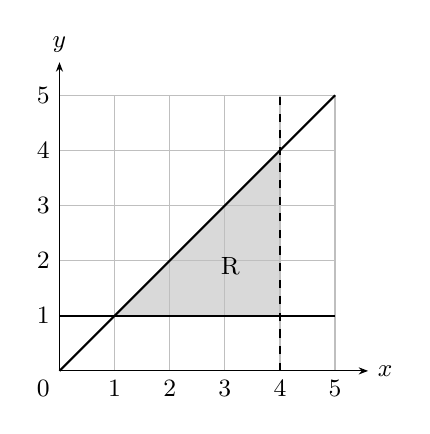
\begin{tikzpicture}[x=7mm,y=7mm,font=\small]
  \fill[black!15] (1,1) -- (4,1) -- (4,4) -- cycle;
  \draw[black!25,step={(1,1)}] (0,0) grid (5,5);
  \draw[-{Stealth[length=1.2mm]}] (0,0) -- (5.6,0) node[right] {$x$};
  \draw[-{Stealth[length=1.2mm]}] (0,0) -- (0,5.6) node[above] {$y$};
  \foreach \t in {1,...,5}{\node[below] at (\t,0) {\t}; \node[left] at (0,\t) {\t};}
  \node[below left] at (0,0) {0};
  \draw[thick] (0,1) -- (5,1);
  \draw[thick,dashed] (4,0) -- (4,5);
  \draw[thick] (0,0) -- (5,5);
  \node at (3.1,1.9) {R};
\end{tikzpicture}
\q Draw a set of axes, with $x$ and $y$ from $-1$ to 5. Shade the region where $x\ge0$, $y\ge1$ and $x+y\le4$. How many points with whole-number coordinates are in the region, including its edges?

% ----------------------------------------------------------------
\topic{Dividing by a negative number}
\q Solve\quad (a) $-2x>8$\qquad (b) $-5x\le-15$\\[2pt]
(c) $7-3x<1$
\q Jo solves $10-2x>4$ and gets $x>3$. Test $x=4$ in $10-2x>4$, and explain Jo's mistake.

% ----------------------------------------------------------------
\topic{Problem solving}
\q Find all the integers that satisfy both $3x-1>5$ and $2x+3\le15$.
\q Write a double inequality whose integer solutions are exactly $-2$, $-1$, 0 and 1.
\q Phone plan A costs £10 a month, plus 5p for each minute of calls. Plan B costs £18 a month, plus 1p for each minute. For how many minutes of calls in a month is plan B cheaper?

\end{multicols}

\end{document}
